\documentclass{article}
\usepackage{mathrsfs}
\usepackage{amsmath}
\usepackage{amsthm}
\usepackage{amssymb}
\usepackage{graphicx}
\usepackage{color}
%\include{macros}
%\usepackage{floatflt}
%\usepackage{graphics}
%\usepackage{epsfig}


\theoremstyle{definition}
\newtheorem{theorem}{Theorem}[section]
\newtheorem{lemma}[theorem]{Lemma}
\newtheorem{proposition}[theorem]{Proposition}
\newtheorem{corollary}[theorem]{Corollary}

\theoremstyle{definition}
\newtheorem*{defition}{Definition}
\newtheorem*{example}{Example}

\theoremstyle{remark}
\newtheorem*{remark}{Remark}
\newtheorem*{note}{Note}
\newtheorem*{exercise}{Exercise}

\setlength{\oddsidemargin}{-0.25 in}
\setlength{\evensidemargin}{-0.25 in} \setlength{\topmargin}{-0.25
in} \setlength{\textwidth}{7 in} \setlength{\textheight}{8.5 in}
\setlength{\headsep}{0.25 in} \setlength{\parindent}{0 in}
\setlength{\parskip}{0.1 in}

\newcommand{\homework}[4]{
\pagestyle{myheadings} \thispagestyle{plain}
\newpage
\setcounter{page}{1} \setcounter{section}{#4} \noindent
\begin{center}
\framebox{ \vbox{\vspace{2mm} \hbox to 6.28in { {\bf
THU-70250043,~Pattern~Recognition~(Spring 2016) \hfill Homework: 2} }
\vspace{6mm} \hbox to 6.28in { {\Large \hfill #1 \hfill} }
\vspace{6mm} \hbox to 6.28in { {\it Lecturer: #2 \hfill} }
\vspace{2mm} \hbox to 6.28in { {\it Student: #3 \hfill} }
\vspace{2mm} } }
\end{center}
\markboth{#1}{#1} \vspace*{4mm} }


\begin{document}

\homework{Parameter Estimation Method}{Changshui Zhang
\hspace{5mm} {\tt zcs@mail.tsinghua.edu.cn}}{ \hspace{5mm} {\tt
 } }{8}

%%%%%%%%%%%%%%%%%%%%%%%%%%%%%%%%%%%%%%%%%%%%%%%%%%%%%%%%%%%%%%%%%%%%
% Section 2.  Problem
%%%%%%%%%%%%%%%%%%%%%%%%%%%%%%%%%%%%%%%%%%%%%%%%%%%%%%%%%%%%%%%%%%%%

\section*{}
1.
\begin{figure}[htbp]
  \centering
  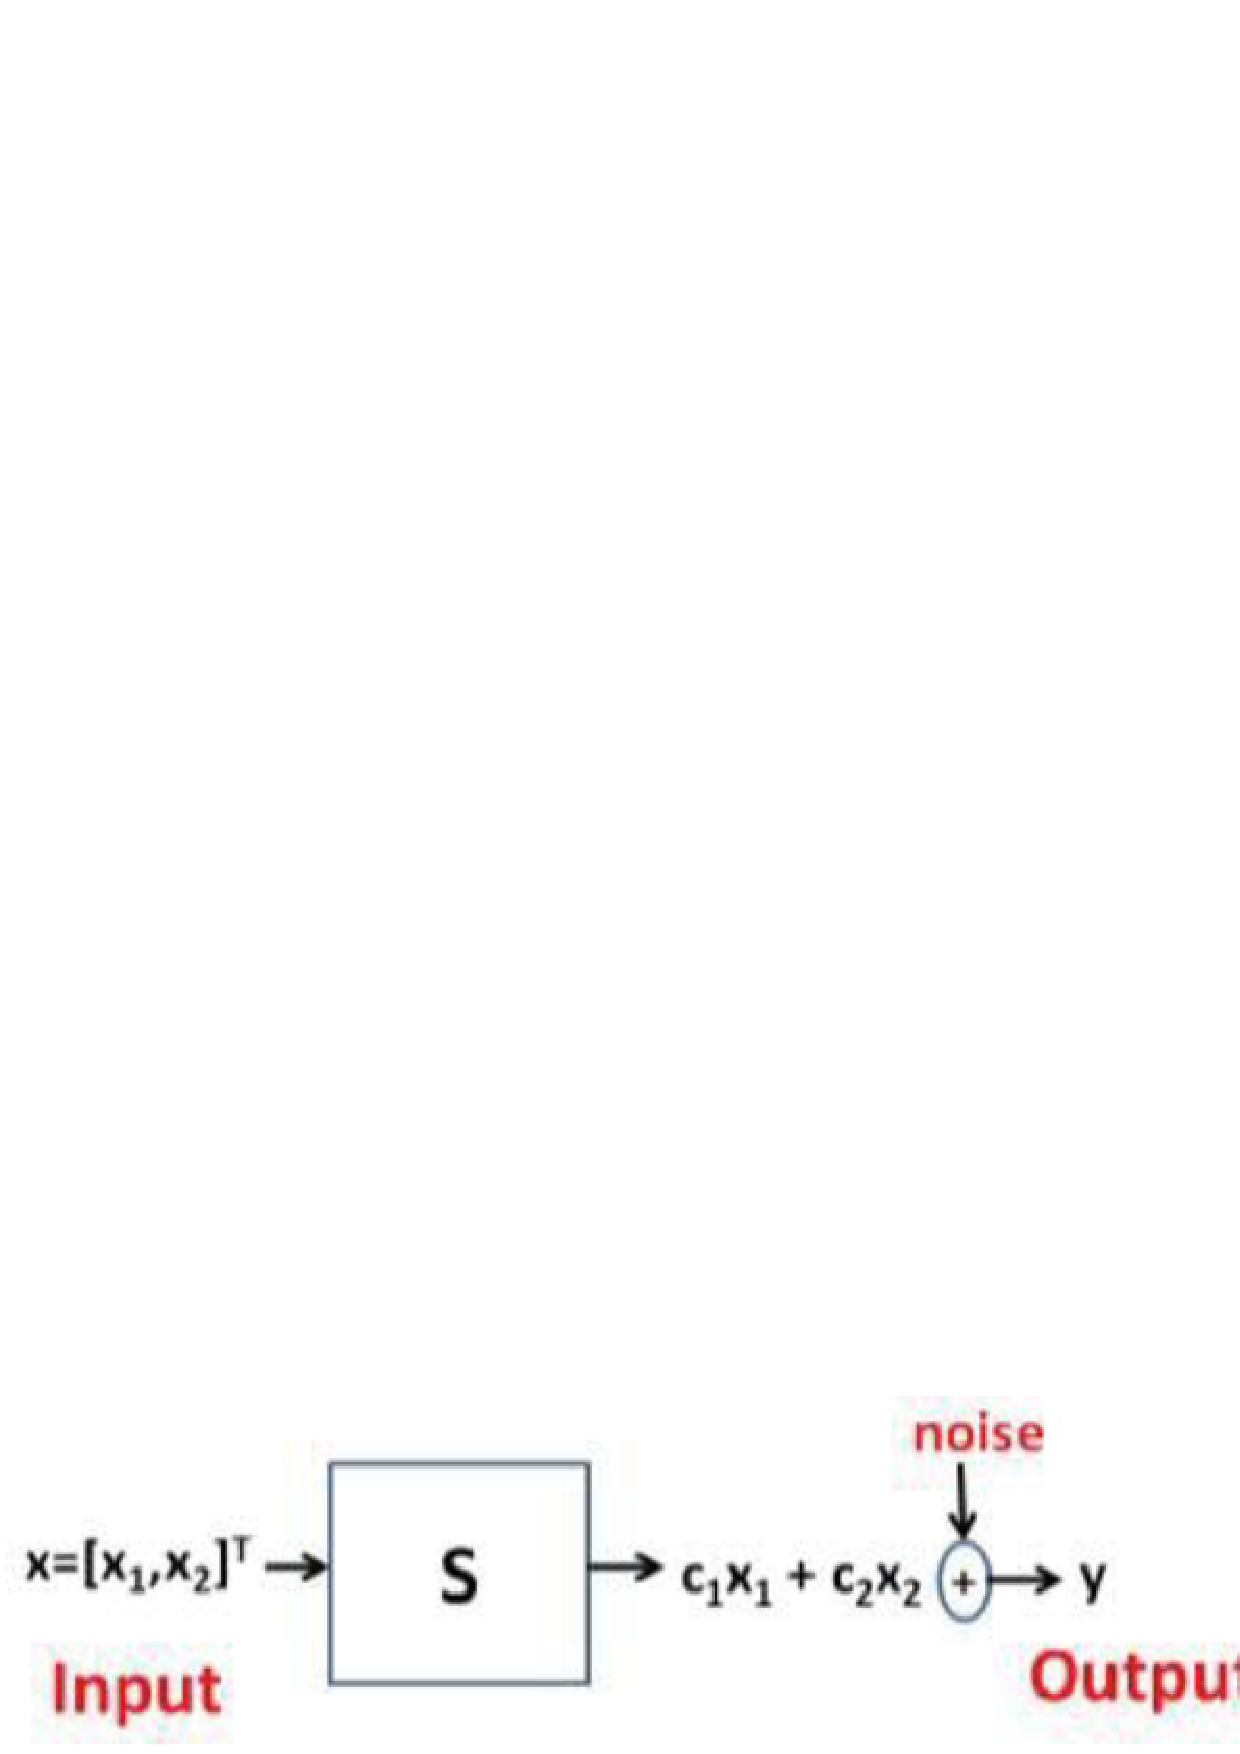
\includegraphics[width=0.35\textwidth]{figure1.png}
  \caption{System S}\label{}
\end{figure}

 Figure 1 shows a system S which takes two inputs $x_1,x_2$(which are deterministic) and outputs a linear combination of those two inputs, $c_1x_1+c_2x_2$, introduces an additive error $\epsilon$ which is a random variable following some distribution. Thus the output $y$ that you observe is given by equation (1). Assume that you have $n>2$ instances $<x_{j1},x_{j2},y_j>_{j=1,...,n}$
$$y=c_1x_1+c_2x_2+\epsilon  \qquad (1)$$
In other words having n equations in your hand is equivalent to having n equations of the following form:$y_j=c_1x_{j1}+c_2x_{j2}+\epsilon _j,j=1,...,n $ The goal is to estimate $c_1,c_2$ from those measurements by maximizing conditional log-likelihood given the input, under different assumptions for the noise. Specifically:

1) Assume that the $\epsilon _i$ for $i=1,...,n$ are iid Gaussian random variables with zero mean and variance $\sigma ^2$.

\qquad (a) Find the conditional distribution of each $y_i$ given the inputs

\qquad (b) Compute the log-likelihood of $y$ given the inputs

\qquad (c) Maximize the likelihood above to get $c_{ls}$


2) Assume that the $\epsilon _i$ for $i=1,...,n$ are independent Gaussian random variables with zero mean and variance $Var(\epsilon _i)=\sigma _i$.

\qquad (a) Find the conditional distribution of each $y_i$ given the inputs

\qquad (b) Compute the log-likelihood of $y$ given the inputs

\qquad (c) Maximize the likelihood above to get $c_{wls}$


3) Assume that the $\epsilon _i$ for $i=1,...,n$ has density $f_{\epsilon_i}(x)=f(x)=\frac{1}{2b}exp(-\frac{|x|}{b})$. In other words our noise is iid following Laplace distribution with location parameter $\mu =0$ and scale parameter $b$.

\qquad (a) Find the conditional distribution of each $y_i$ given the inputs

\qquad (b) Compute the log-likelihood of $y$ given the inputs

\qquad (c) Comment on why this model leads to more robust solution.


2.  Consider a normal $p(x)\sim N(\mu,\sigma^2)$ and Parzen-window function $\phi(x)\sim N(0,1)$ Show that the Parzen-window estimate
$$
p_n(x) = \frac{1}{nh_n}\sum_{i=1}^{n}\phi(\frac{x-x_i}{h_n})
$$
has the following properties:

(a)$\overline{p}_n(x)\sim N(\mu,\sigma^2+h_n^2)$

(b)$Var[p_n(x)] \simeq \frac{1}{2nh_n\sqrt{\pi}}p(x)$

(c)$p(x)-\overline{p}_n(x)\simeq \frac{1}{2}(\frac{h_n}{\sigma})^2[1-(\frac{x-\mu}{\sigma})^2]p(x)$ for small $h_n $

(Note: if $h_n = \frac{h_1}{\sqrt n} $, this show that the error due to bias goes to zero as $1/n $ , whereas the
standard deviation of the noise only goes to zero as ${\sqrt[4]{n}} $.)


3.  One measure of the difference between two distributions in the same space is the
Kullback-Leibler divergence of Kullback-Leibler "distance":

$$
D_{KL}(p_1(x),p_2(x)) = \int p_1(x)ln\frac{p_1(x)}{p_2(x)}dx
$$


(This "distance" does not obey the requisite symmetry and triangle inequalities for a metric.)Suppose we seek to approximate an arbitrary distribution $p_2(x)$ by a normal $p_1(x)\sim N(\mu,\Sigma)$ .
Show that the values that lead to the smallest Kullback-Leibler divergence are the obvious ones:

$$
\mu = \epsilon_2[x]
$$
$$
\Sigma = \epsilon_2[(x-\mu)(x-\mu)^T]
$$

where the expectation $\epsilon_2$ taken is over the density $p_2(x)$.


4. (Programming) Assume  $p(x)\sim0.1N(-1,1)+0.9N(1,1)$.  Draw n samples from $p(x)$, for example, $n=5,10,50,100,\cdots,1000,\cdots,10000$. Use Parzen-window method to estimate $p_n(x)\approx p(x)$ (Hint: use randn() function in matlab to draw samples)

(a) Try window-function $P(x)=\left\{
\begin{aligned}
&\frac{1}{a},-\frac{1}{2}a\leq x\leq \frac{1}{2}a \\
&0,otherwise.
\end{aligned}
\right.$. Estimate $p(x)$ with different window width $a$.

(b)Derive how to compute $\epsilon(p_n)=\int[p_n(x)-p(x)]^2dx$ numerically.

(c)Demonstrate the expectation and variance of $\epsilon(p_n)$ w.r.t different $n$ and $a$ .

(d)With n given, how to choose optimal $a$ from above the empirical experiences?

(e)Substitute $h(x)$ in (a) with Gaussian window. Repeat (a)-(e).

(g)Try different window functions and parameters as many as you can. Which window
function/parameter is the best one? Demonstrate it numerically.



%%%%%%%%%%%%%%%%%%%%%%%%%%%%%%%%%%%%%%%%%%%%%%%%%%%%%%%%%%%%%%%%%%%%
% Reference
%%%%%%%%%%%%%%%%%%%%%%%%%%%%%%%%%%%%%%%%%%%%%%%%%%%%%%%%%%%%%%%%%%%%
%\begin{thebibliography}{1}

%\bibitem{BoydVandenberghe2004}
%S. Boyd and L. Vandenberghe, \emph{Convex Optimization}, Cambridge
%University Press, 2004.

%\end{thebibliography}
\end{document}
